\documentclass[10pt]{standalone}
\usepackage{commands}

\begin{document}
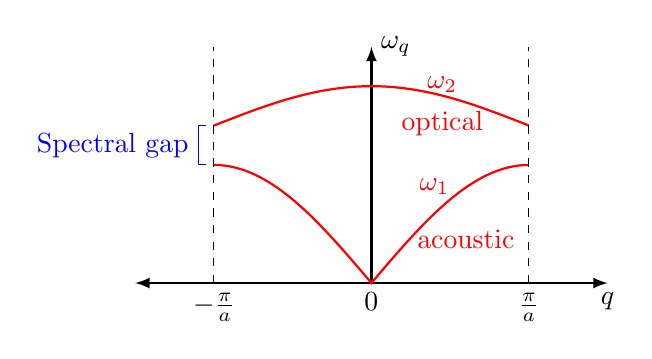
\begin{tikzpicture}
    \draw[-latex, thick] (0, 0) -- (0, 3);
    \draw[latex-latex, thick] (-3, 0) -- (3, 0);
    \node[below] at (3, 0) {$q$};
    \node[right] at (0, 3) {$\omega_q$};
    \draw[red, thick] (-2, 1.5) cos (0, 0) sin (2, 1.5);
    \draw[red, thick] (-2, 2) sin (0, 2.5) cos (2, 2);
    \draw[dashed] (-2, 0) -- (-2, 3);
    \draw[dashed] (2, 0) -- (2, 3);
    \node[below] at (0, 0) {0};
    \node[below] at (-2, 0) {$-\frac{\pi}{a}$};
    \node[below] at (2, 0) {$\frac{\pi}{a}$};
    \node[red, above] at (0.8, 1) {$\omega_1$};
    \node[red, below] at (1.2, 0.8) {acoustic};
    \node[red, above] at (0.9, 2.3) {$\omega_2$};
    \node[red, below] at (0.9, 2.3) {optical};
    \draw[blue] (-2.1, 1.5) -- (-2.2, 1.5) -- (-2.2, 2) -- (-2.1, 2);
    \node[blue, left] at (-2.2, 1.75) {Spectral gap};
\end{tikzpicture}
\end{document}